\documentclass{article}
\usepackage[utf8]{inputenc}
\usepackage{graphicx}
\usepackage{grffile}   
\usepackage{float}
\usepackage{amsmath,amssymb}
\renewcommand{\thesubsection}{\thesection.\alph{subsection}}
\usepackage{caption}
\usepackage{subcaption}



%Images 

%\begin{figure}[H]
%    \centerline{\includegraphics[scale=0.6]{images/image_Q1_ii.pdf}}
%    \caption{The error in differentiation schemes as a function of h.}
%    \label{fig:1d}
%\end{figure}
\begin{document}



\title{PHY407 Lab10}
\author{Genevieve Beauregard (1004556045)\\ Anna Shirkalina (1003334448)}
\date{Oct 2020}
\maketitle


\section*{Q1}
\subsection*{a)}
We are asked to implement the simulated annealing optimiziation for the walking salesman problem. Using the \texttt{salesman.py} code from Newman we adjust the algorith to account for multiple trials and our desired seeding method as described in the lab manual. We start each simulation with the dots arranged as in figure \ref{fig:1a_original}.

 \begin{figure}[H]
     \centerline{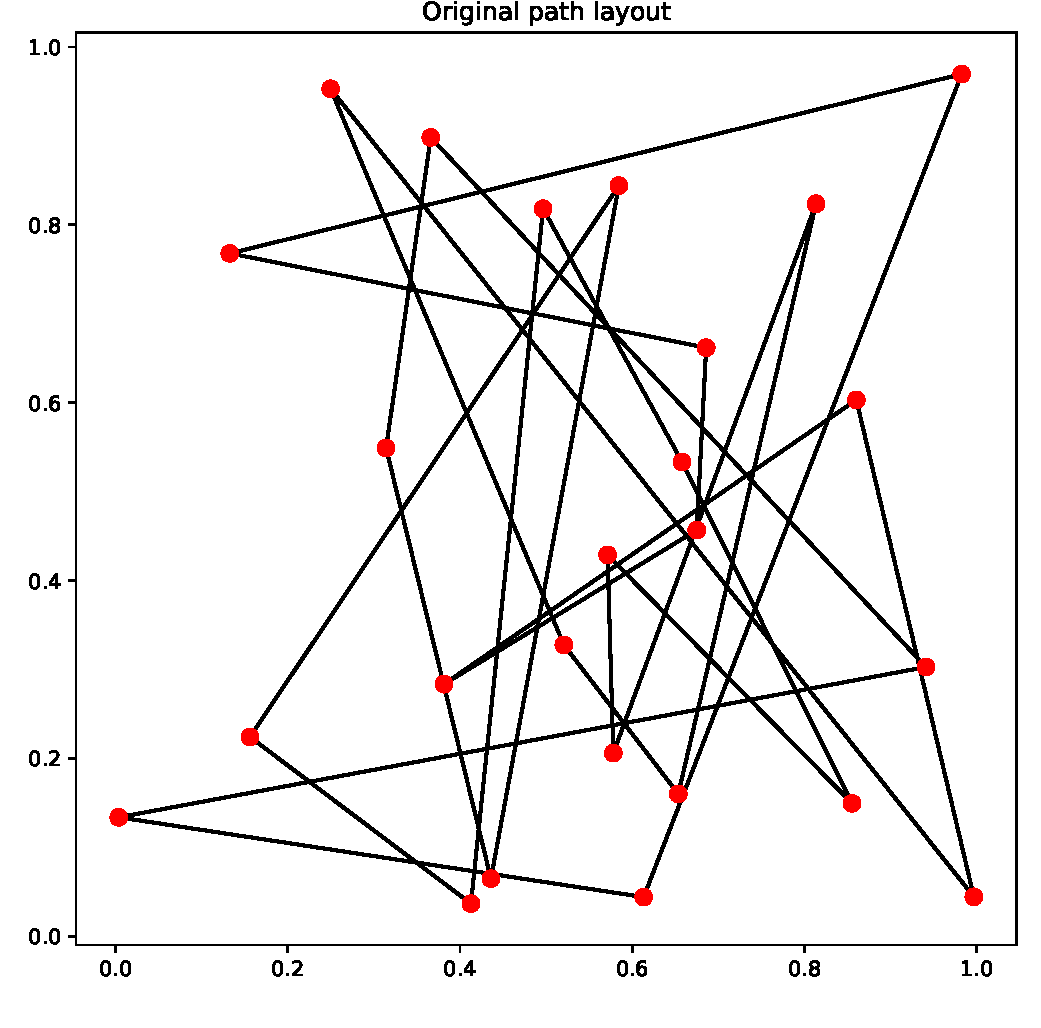
\includegraphics[scale=0.6]{images/Q1a_path0_tau10000.pdf}}
     \caption{The original layout of the dots for each simulation.}
     \label{fig:1a_original}
 \end{figure}
 \begin{figure}[H]
     \centerline{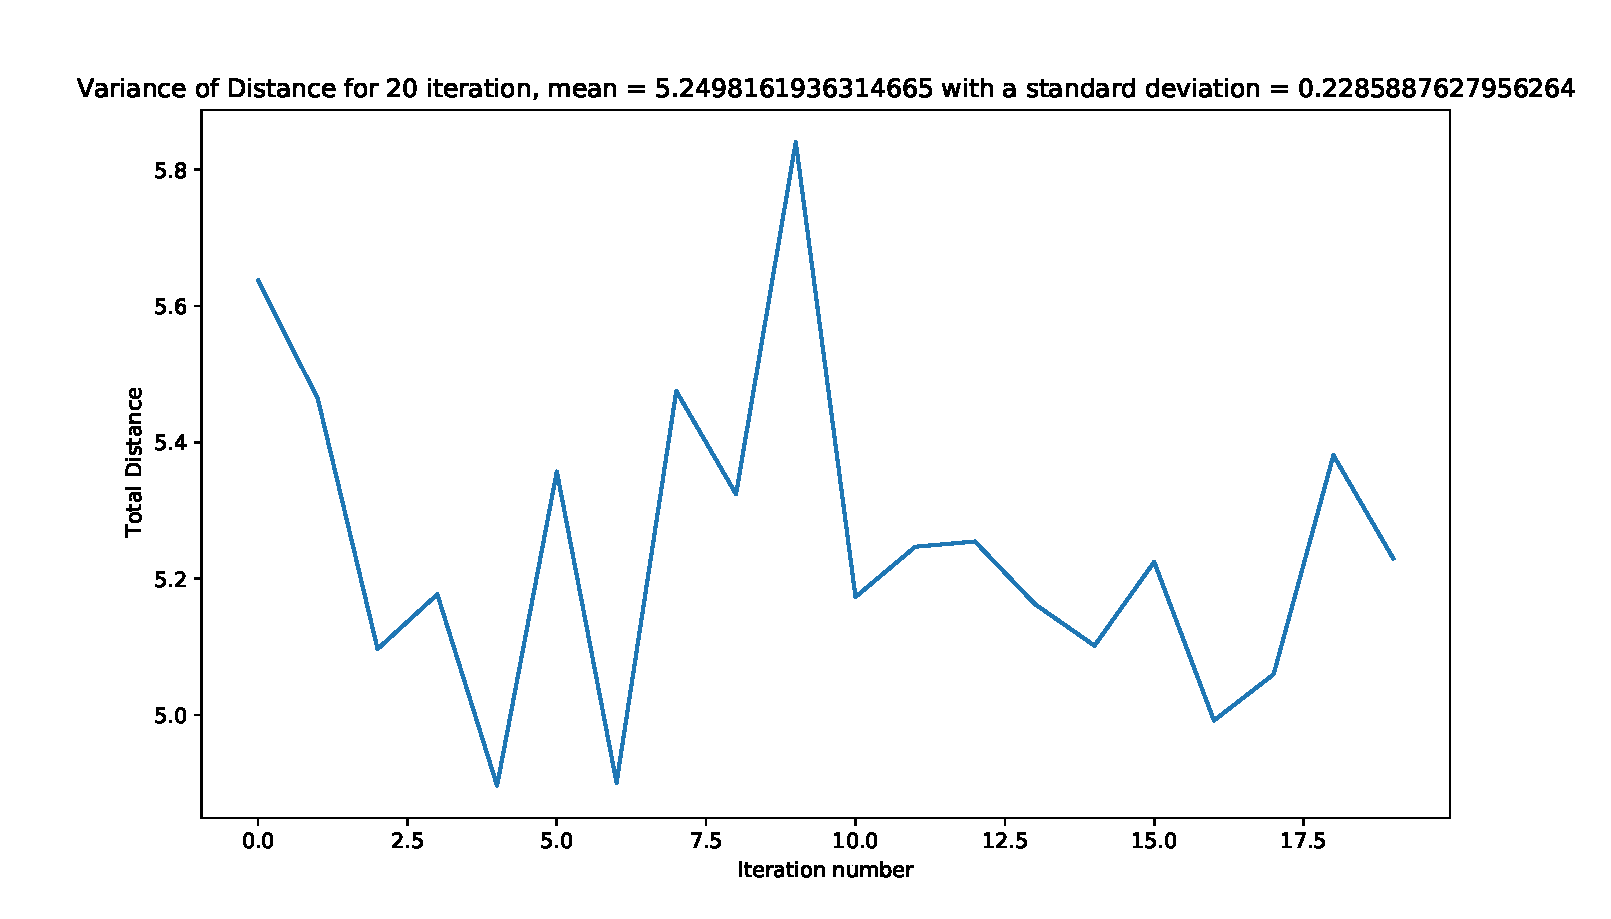
\includegraphics[scale=0.6]{images/Q1a_distances_tau10000.pdf}}
     \caption{The distances over 20 simulations at tau =10000.}
     \label{fig:1a_distances_tau10000}
 \end{figure}
 \begin{figure}[H]
     \centerline{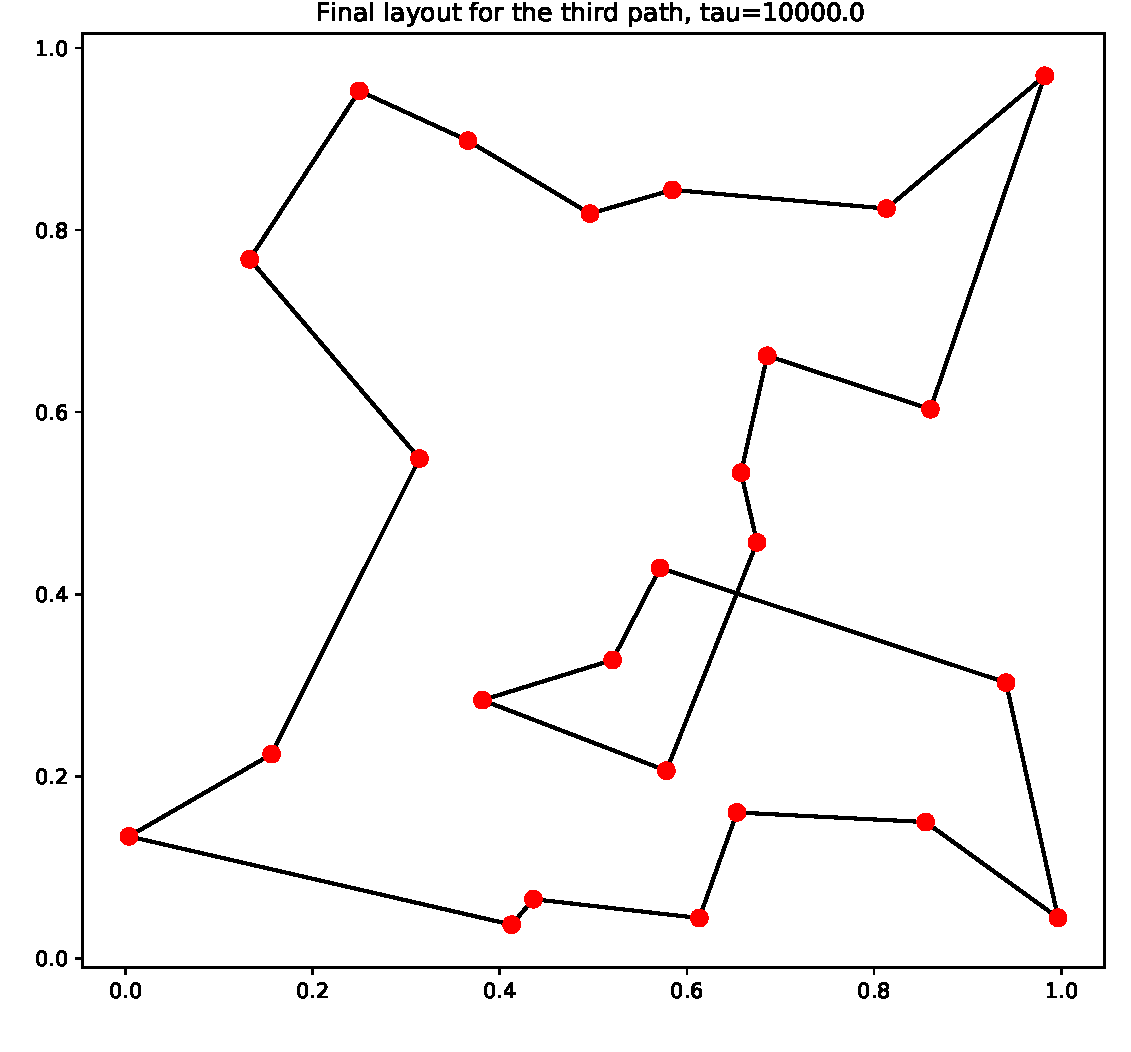
\includegraphics[scale=0.6]{images/Q1a_path3_tau10000.pdf}}
     \label{fig:1a_path3_tau10000}
 \end{figure}
 \begin{figure}[H]
     \centerline{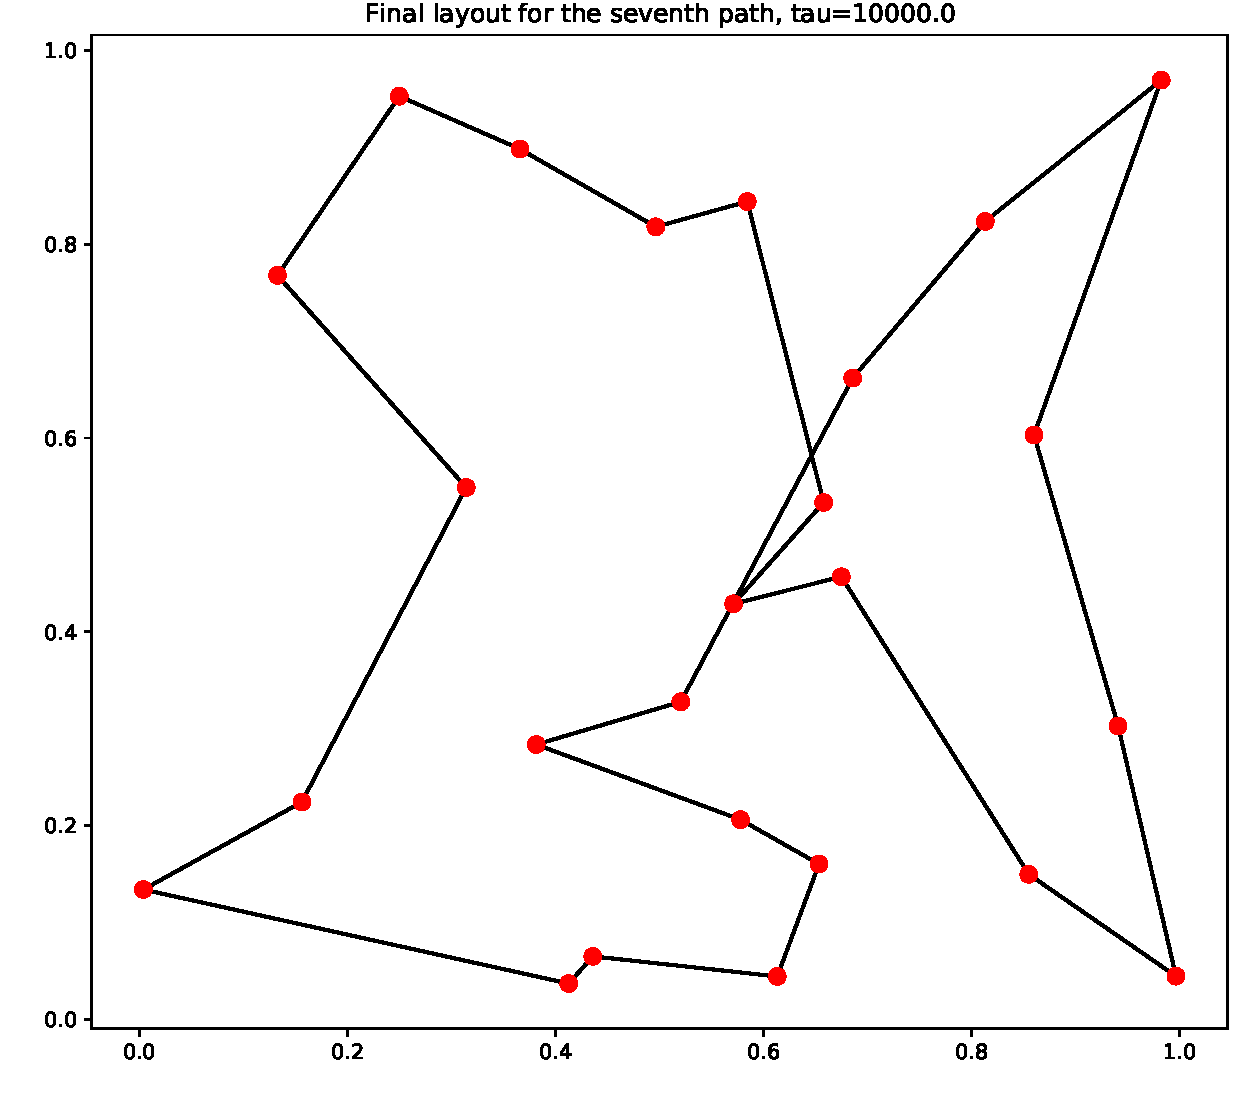
\includegraphics[scale=0.6]{images/Q1a_path7_tau10000.pdf}}
     \label{fig:1a_path7_tau10000}
 \end{figure}
 \begin{figure}[H]
     \centerline{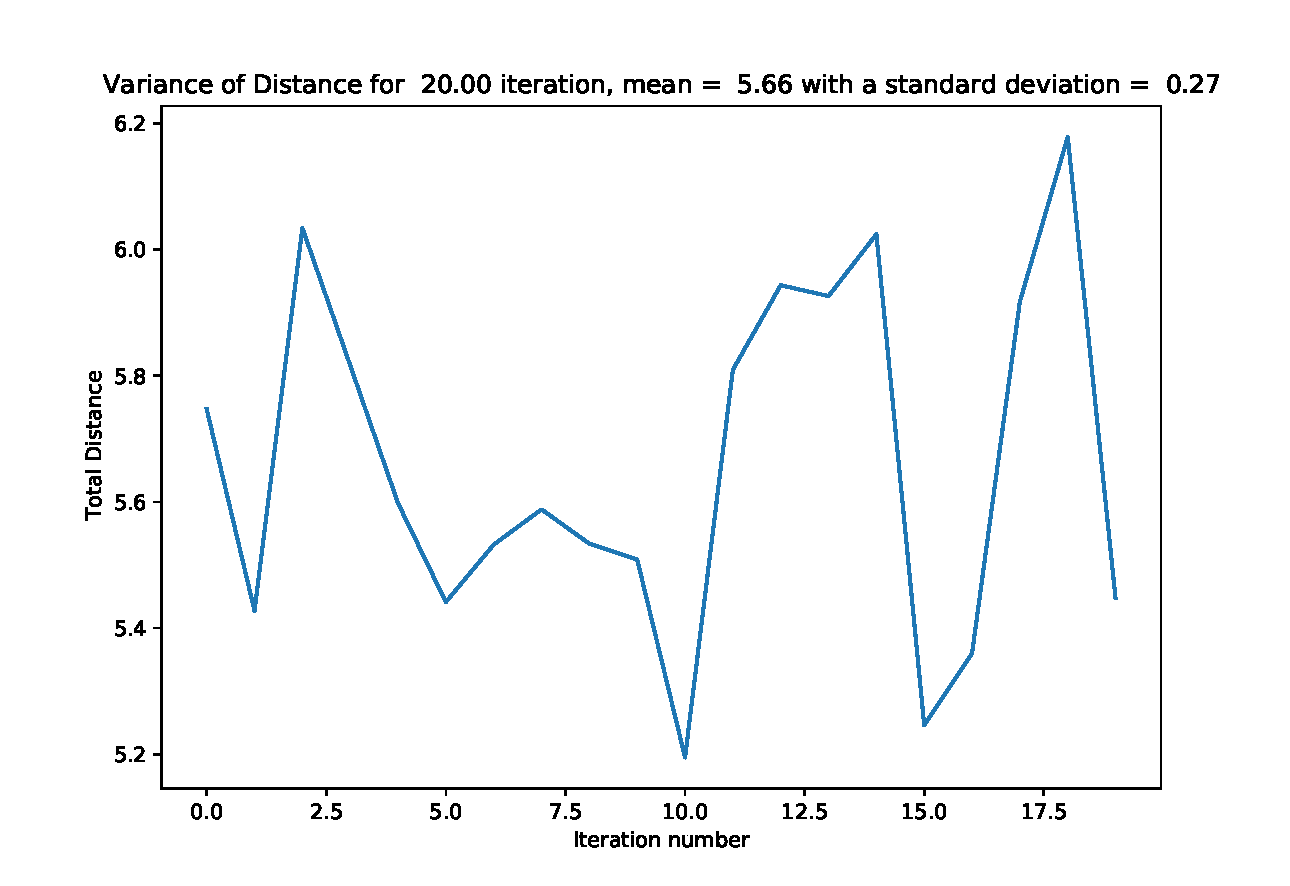
\includegraphics[scale=0.6]{images/Q1a_distances_tau1000.pdf}}
     \caption{The distances over 20 simulations at tau =1000.}
     \label{fig:1a_distances_tau1000}
 \end{figure}
 \begin{figure}[H]
     \centerline{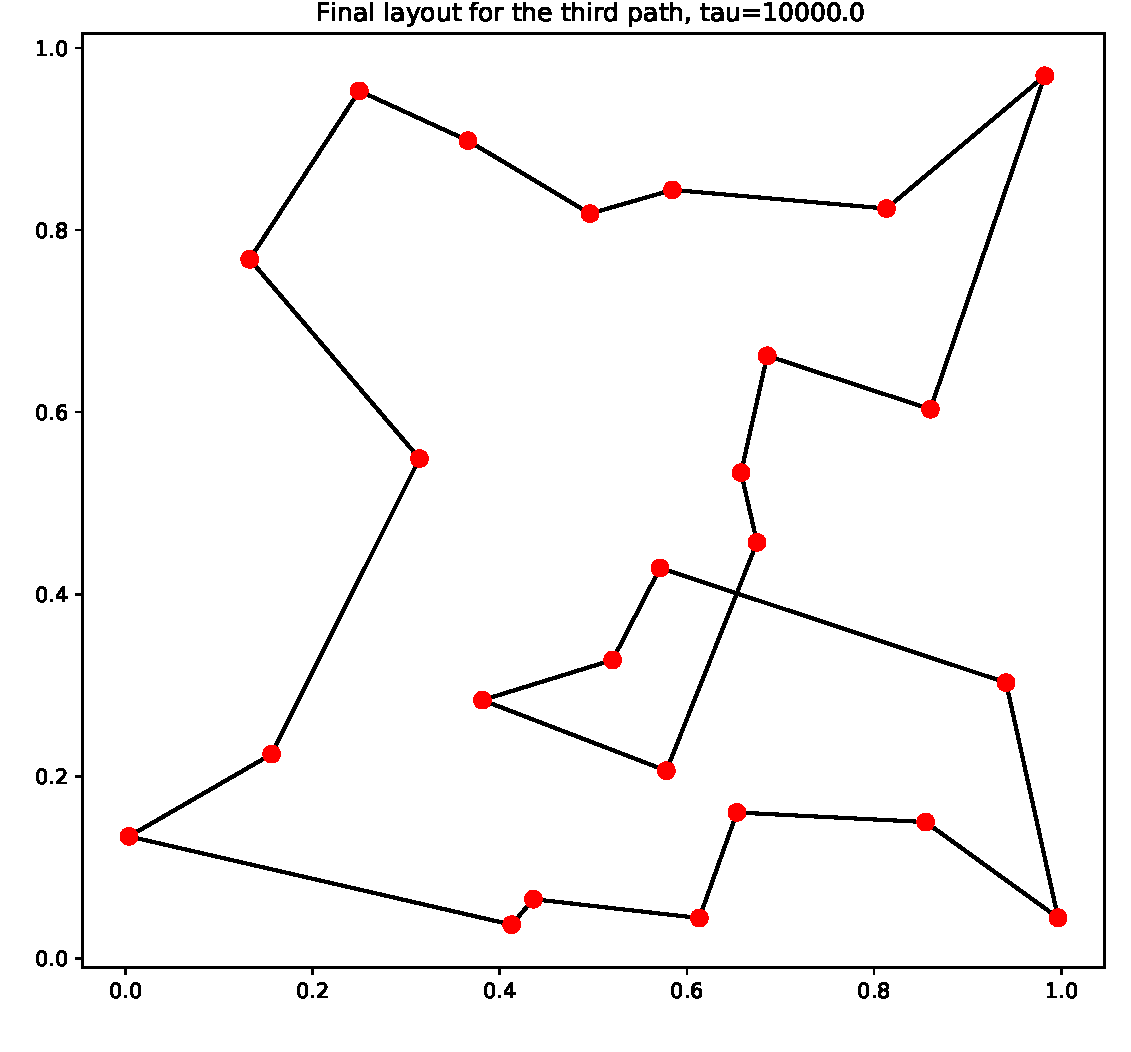
\includegraphics[scale=0.6]{images/Q1a_path3_tau10000.pdf}}
     \label{fig:1a_path3_tau1000}
 \end{figure}
 \begin{figure}[H]
     \centerline{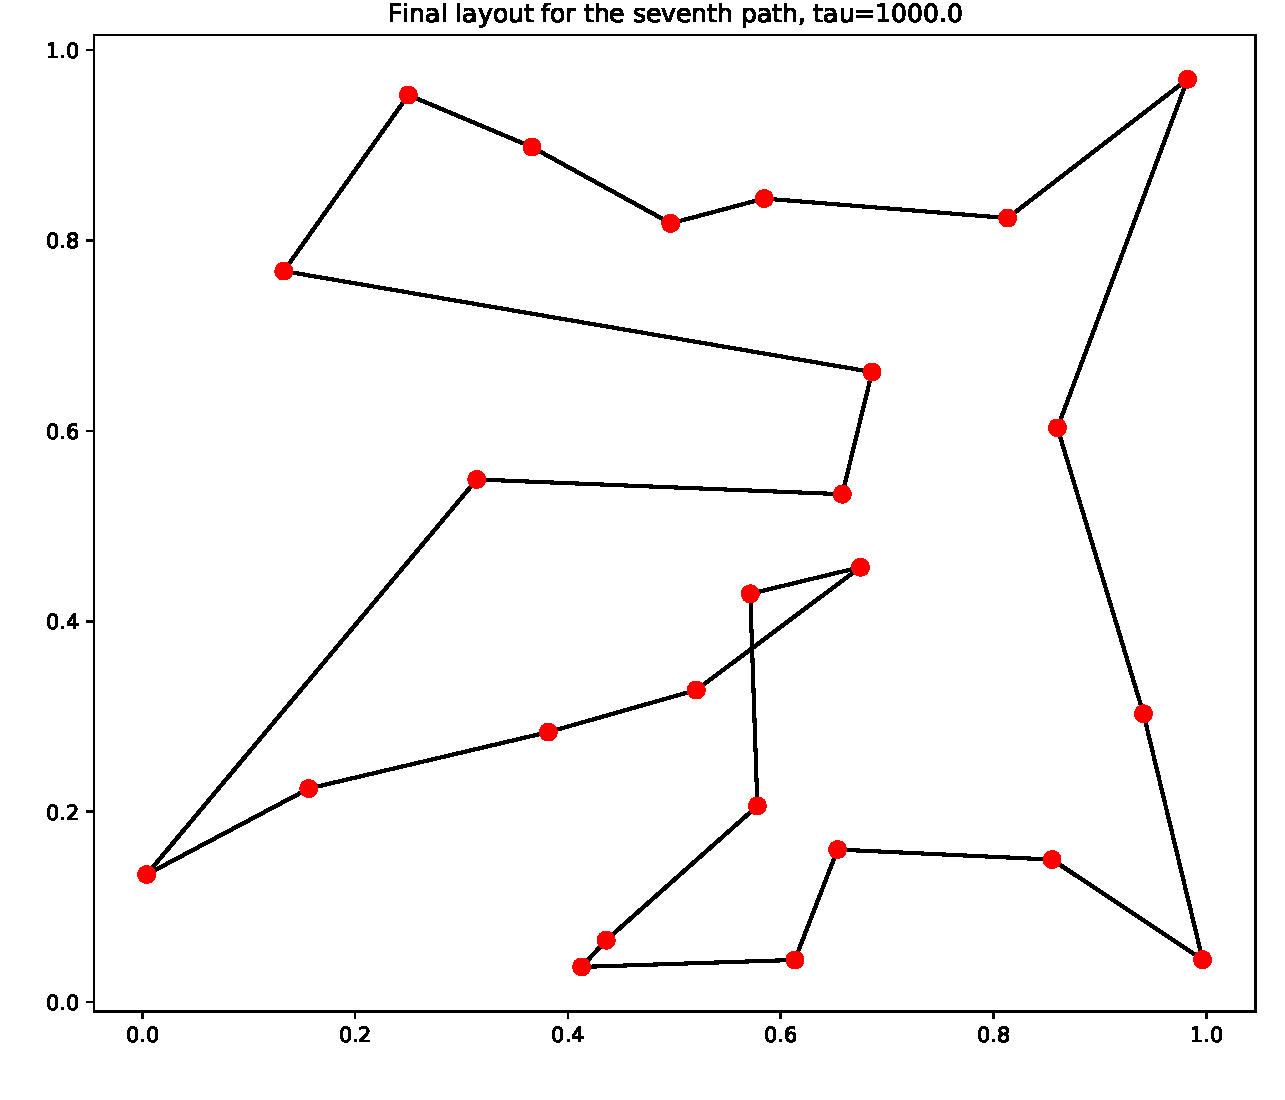
\includegraphics[scale=0.6]{images/Q1a_path7_tau1000.pdf}}
     \label{fig:1a_path7_tau1000}
 \end{figure}

\subsection*{b)}
\subsubsection*{i)}
We are asked to implement a simulated annealing algorithm to find the global maximum of $f(x, y) = x^2 - cos(4 \pi x) + (y - 1)^2$. As suggested we use an exponential cooling schedule and exponential constant. We plot the values of x, y over time in figure \ref{fig:1bi}. We find that 
\begin{verbatim}
    Tmax = 10.0
    Tmin = 1e-3
    tau = 1e3    
\end{verbatim}
are sufficient constants to arrive at an appropriate guess in an appropriate amount of time in our program. Our program predicts in 9211 iterations that the minimum is at (0.007191847797809098, 0.961920529983146) which is sufficiently close to the analytical minimum. 


\begin{figure}[H]
    \centerline{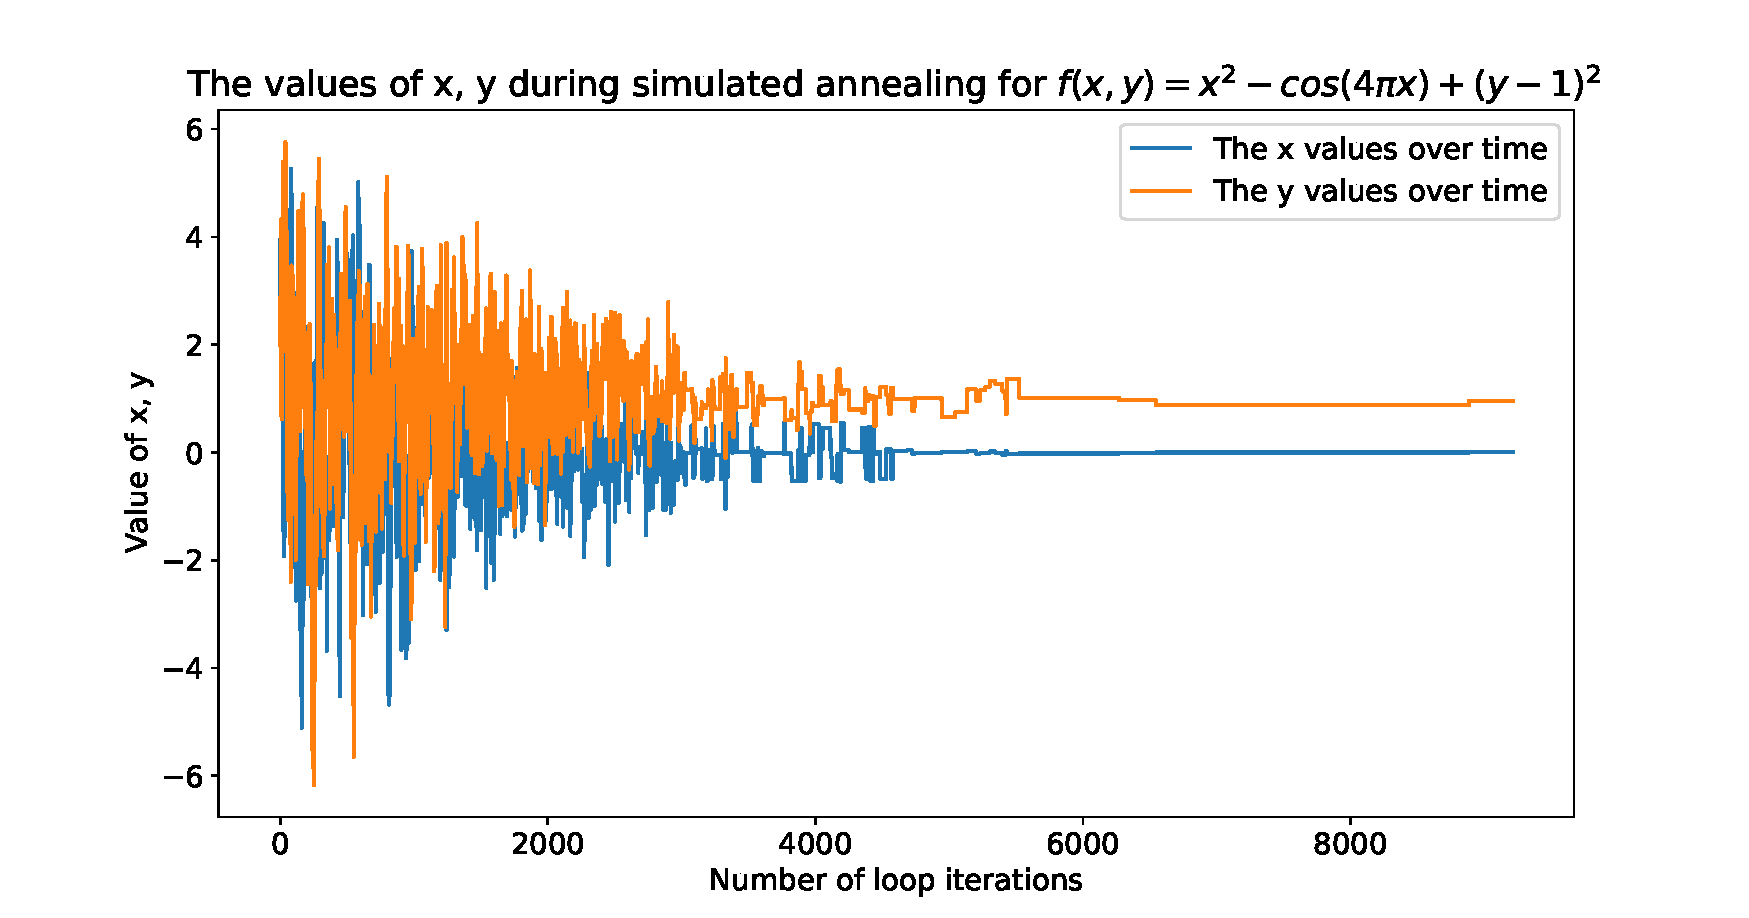
\includegraphics[scale=0.6]{images/Q1bi.pdf}}
    \caption{The predicted values of x, y over the iterations run in the program for $f(x, y) = x^2 - cos(4 \pi x) + (y - 1)^2$.}
    \label{fig:1bi}
\end{figure}


\subsubsection*{ii)}
We are asked to implement a simulated annealing algorithm to find the global maximum of $f(x, y) = cos(x) + cos(\sqrt{2} x)+ cos(\sqrt{3} x) + (y - 1)^2$. As suggested we use an exponential cooling schedule and exponential constant. We plot the values of x, y over time in figure \ref{fig:1bii}. We find that 
\begin{verbatim}
    Tmax = 10.0
    Tmin = 1e-3
    tau = 1e35   
\end{verbatim}
are sufficient constants to arrive at an appropriate guess in an appropriate amount of time in our program. Our program predicts in 921035 iterations that the minimum is at (15.937357585687492, 0.9897636033808369) which is sufficiently close to the analytical minimum. If the script is run multiple times we find that on occasion we instead find one of the suggest competing minimums at $y = 1, x =\approx 2, x \approx 46$. 

\begin{figure}[H]
    \centerline{\includegraphics[scale=0.6]{images/Q1bii.pdf}}
    \caption{The error in differentiation schemes as a function of h.}
    \label{fig:1bii}
\end{figure}

Tmax = 10.0
Tmin = 1e-3
tau = 1e5


\newpage
\section*{Q2)}
Here, we are instructed to build a Metropolis-like algorithm for the Ising Model. We are asked to consider a 20x20 array grid of random spin up or down states, represented by $\pm 1$. Energy of this state is calculated as follows: 
\[E = J \sum_{\langle i, j \rangle} s_i s_j \]
where $s_i$ and $s_j$ are adjacent pairs in the grid. 

The magnetism is calculated as the sum of the dipoles in the grid, 
\[ M = \sum_{i} s_i \]

We randomly flip one of the dipoles state to obtain a $E_{new}$ state.

The Boltzman factor for this  $E_{new}$ from $E_{old}$ is 
\[ p = \exp(-(E_{new} - E_{old})/k_B T) \]

\subsection*{a)}
We adapt the function \texttt{energyfunction} from the starter code given in \newline \texttt{L11-Ising1D-start.py} to handle 2-dimensional arrays. To calculate adjacent pairs, we handle the differences in arrays: first multiplying the [i +1] columns with the [i] columns, and then doing the same with rows. More details can be seen in the code. 

\subsection*{b)}
We are instructed to create a Metropolis style algorithm of the Ising model, with $J = 1$, $k_B = 1$ and $T = 1$. 

We first create the function \texttt{acceptance} which returns the boolean value True is the transmission from $E_{old}$ to $E_{new}$ is accepted. We accept $E_{new}$ if the following conditions are met: 
\begin{enumerate}
    \item if $E_{new} - E_{old} <= 0$
 \item if $E_{new}-E_{old} > 0$ and $p > \texttt{random()}$
 
\end{enumerate}

We can calculate the magnetization of a dipole array by simply using \texttt{np.sum(dipoles)}.


\subsubsection*{Pseudocode}
\begin{verbatim}
Def energyfunction(J, dipoles):
    returns E
    
Def acceptance(E_new,E, kB, T): 
    accepted = False
    calculate p 
    if p > random(): 
        accepted = True 
    returns accepted

Initialize kB, T, J
Set number of steps 

Initialize N, grid size
Initialize empty dipole NxN array 
Loop over entries of dipole to populate with +/- 1 entries 

Initialize empty energy, magnetization, dipole_array accumulator lists 
Calculate current energy, magnetization using current dipole value 
Append to respective lists

For range(steps): 
    Pick random coordinate in dipole, and flip spin
    Compute new energy 
    
    Calculate acceptance 
    
    if accepted: 
        append new dipole array, energy and magnetization
    
    if not accepted: 
        flip back spin to original state
        append old E, magnetization and dipoles to respective lists

Plot E, M against steps
Plot dipoles 
\end{verbatim}

\subsection*{c)}
% We run this for $100,000$ steps as instructed in the handout. For this particular run, we get the following plots for magnetization and energy in Fig \ref{fig:q2c_magnet} and Fig \ref{fig:q2c_energy}. We see that all the dipoles would align (or almost completely do so save for a few random cases), developing complete magnetization. Our units are scaled such that $kB = 1, J = 1$.

\begin{figure}[H]
    \centerline{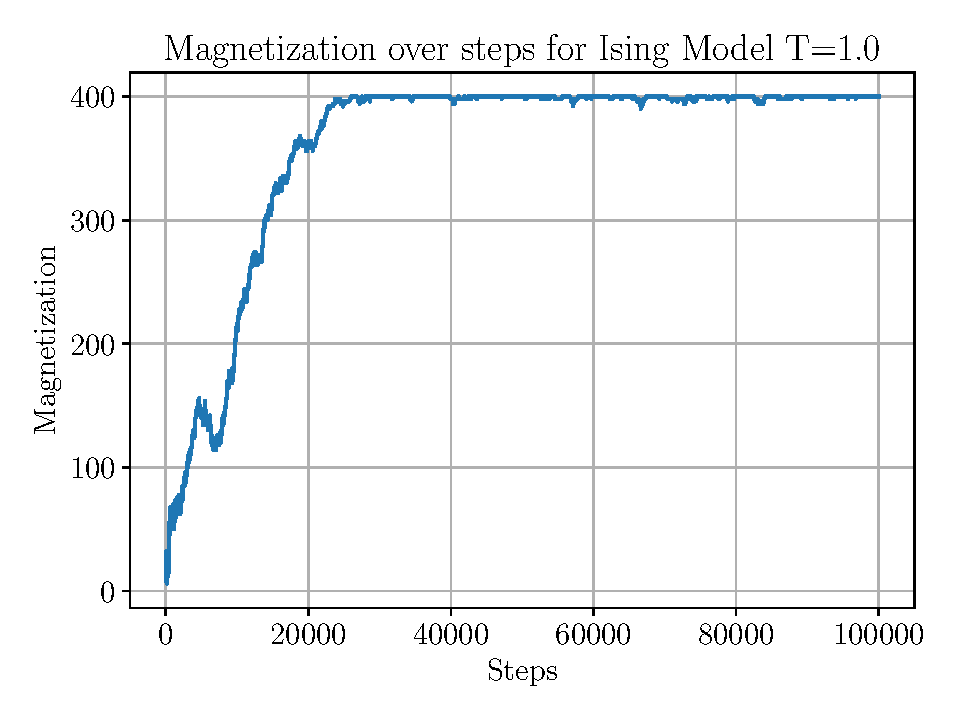
\includegraphics[scale=0.75]{images/Q2_magnetizationT_1.0.pdf}}
    \caption{The Magnetization over the number of steps. This is the same run as Fig \ref{fig:q2c_energy}, we see it converging to 400 (only possible if every dipole is +1)}.
    \label{fig:q2c_magnet}
\end{figure}

\begin{figure}[H]
    \centerline{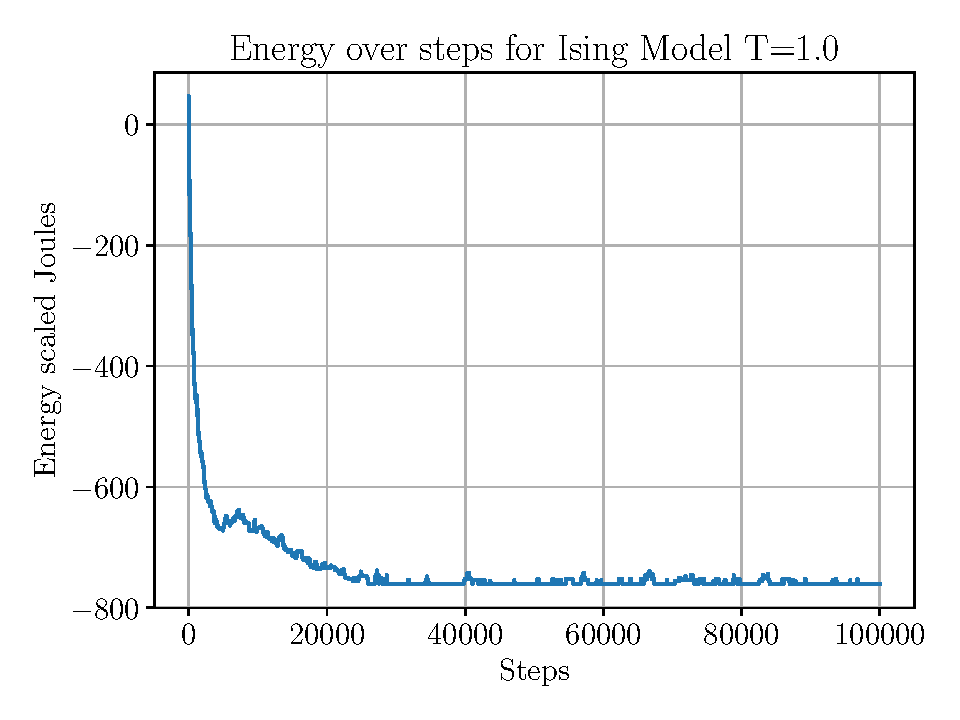
\includegraphics[scale=0.75]{images/Q2_energy_T_1.0.pdf}}
    \caption{The energy over the number of steps. This is the same run as Fig \ref{fig:q2c_magnet}. We see the energy converges to its ground state as expected.}
    \label{fig:q2c_energy}
\end{figure}


\subsection*{d)}
We run our program for a couple of times (we note in some very edge cases, the magnetization occasionally does not converge under 100,000 steps; this may be due randomness). We placed the plots in the appendix, in Fig \ref{fig:q2d_magnet_1} to FIg \ref{fig:q2d_magnet_3}.


We can see there is a tendency for the magnetization to converge to $+400$ or $-400$ as we enter the ground state. This can only occur if all 400 spins we are considering are either positive or negative; the magnetization generally tends towards a case where all spins are in the same direction. This may occur as this is the energetically lowest state of the system, and the boltzman probability is sufficiently low for the routine to bring us to accept higher energies.


\subsection*{e)}
To animate, we use \texttt{FuncAnimation} from \texttt{Matplotlib.animation} module. We plot every 100 frames, with a frame interval of \SI{200}{ms}. 

We animated the $T=1$ case. Our animation is in \texttt{Q2e\_AnimationT1.mp4}. We see that the spins orient themselves quickly; by $t = 1:30 \SI{}{s}$ mark, the spins have all aligned to the $-1.0$. We can see this in the associated plot for magnetization in this run in Fig \ref{fig:q2e_magnet_1}, where the magnetization initially fluctuates but then converges to -400, a state only possible with all spins aligned in -1.0. 
\begin{figure}[h!]
    \centerline{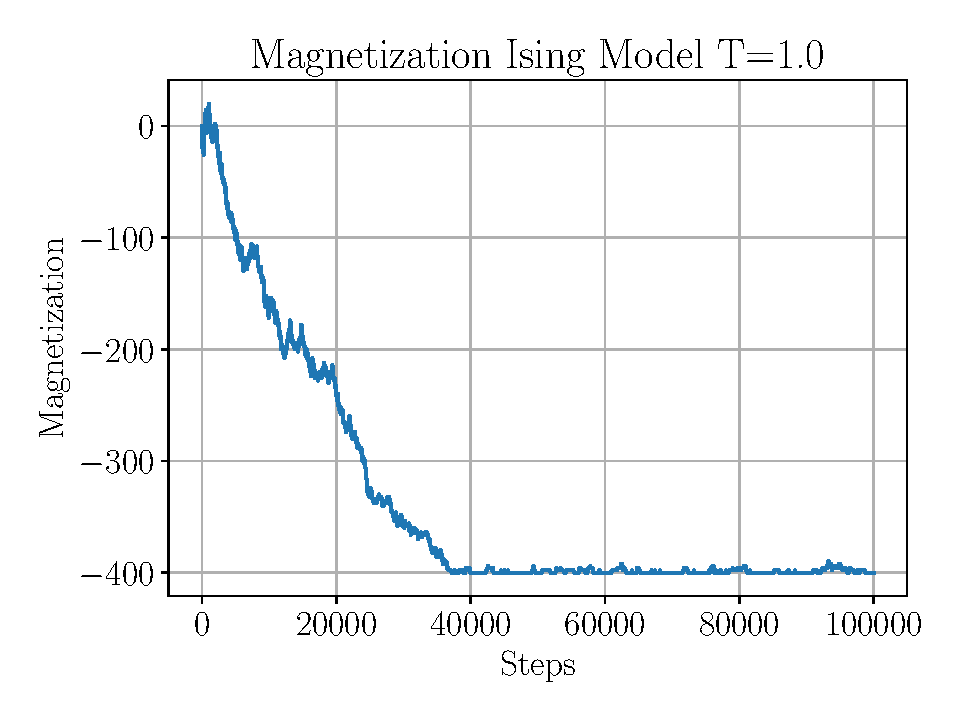
\includegraphics[scale=0.6]{images/Q2e_magnetizationT_1.0.pdf}}
    \caption{Magnetization associated with \texttt{Q2e\_AnimationT1.mp4}, where T =1.0}.
    \label{fig:q2e_magnet_1}
\end{figure}

We animated the $T=2$ case. Our animation is in \texttt{images/Q2e\_AnimationT2.mp4}. We see that the spins do not collectively converge to a state where they all align. There appears to be some alignment occurring with some small pockets having all the spins either aligned up or down. At certain points, we see large areas +1 spin. We can see that behaviours being reflected in the Magnetization of this run; we plotted this in Fig \ref{fig:q2e_magnet_2}. The magnetization appears to fluctuate about 150/200 consistent with the larger pockets of +1 spins occurring in the animation at certain points. 
\begin{figure}[h!]
    \centerline{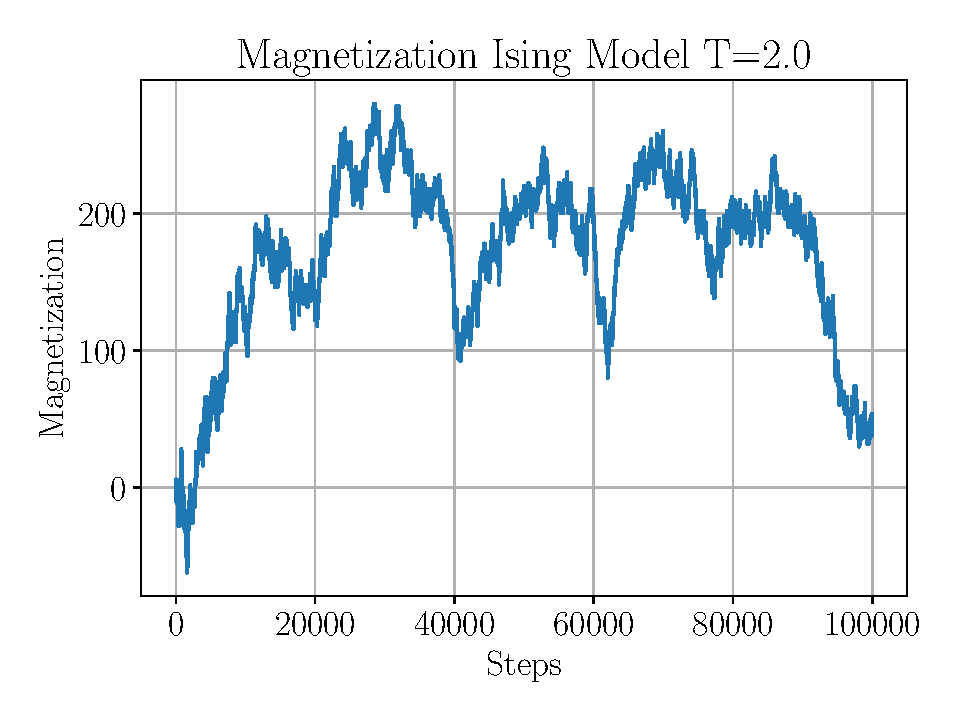
\includegraphics[scale=0.6]{images/Q2e_magnetizationT_2.0.pdf}}
    \caption{Magnetization associated with \texttt{Q2e\_AnimationT2.mp4}, where $T =2.0$.}.
    \label{fig:q2e_magnet_2}
\end{figure}

We animated the $T=3$ case. Our animation is in \texttt{Q2e\_AnimationT3.mp4}. We see that the spins do not collectively converge to a state where they all align. In this case, the spins behaviour is mostly chaotic with only very local spin alignment occurring. There appears to be no convergent behaviour. We can see that behaviours being reflected in the Magnetization of this run; we plotted this in Fig \ref{fig:q2e_magnet_3}. 
\begin{figure}[h!]
    \centerline{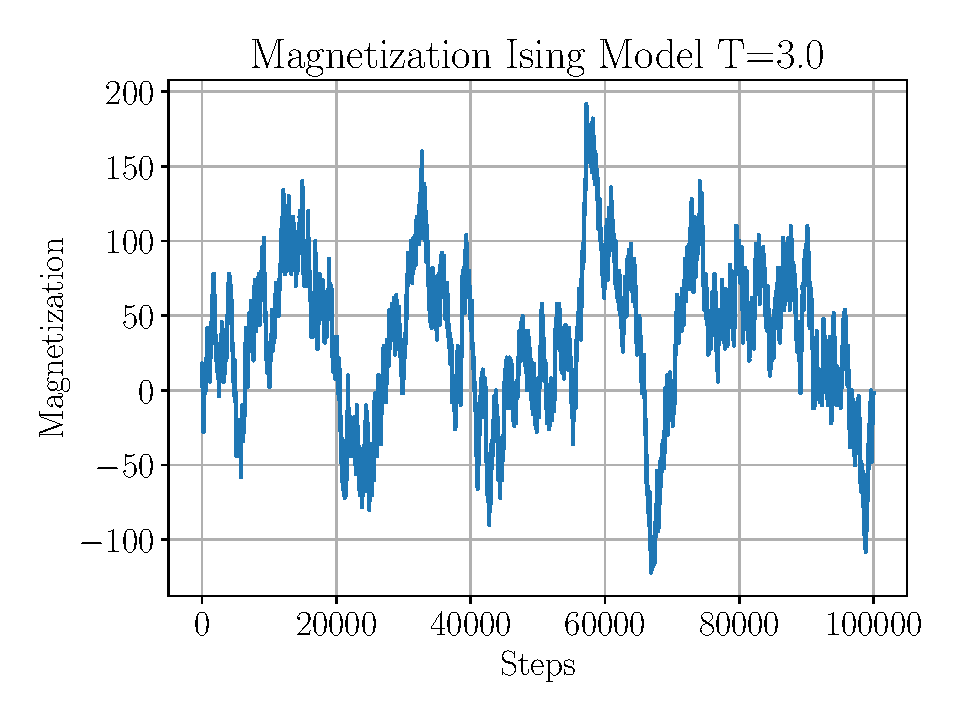
\includegraphics[scale=0.6]{Q2e_magnetizationT_3.0.pdf}}
    \caption{Magnetization associated with \texttt{Q2e\_AnimationT3.mp4}, where $T =3.0$.}
    \label{fig:q2e_magnet_3}
\end{figure}
\newpage
\hfill
\newpage

\section*{Q3}
% blurb here describing the physics 


\subsection*{a)}
We are asked to run the provided script \texttt{L11-Qprotein-start.py} with the default parameters $N = 30$, $T =1.5$, $\epsilon = -5$, $n = 10^5$. The script returns two figures - one of the final structure of the protein and one that shows the energy as a function of steps. We run the script as instructed as obtain plots as seen in Fig \ref{fig:q3a_protein1} and \ref{fig:q3a_energy1}. \\
\begin{figure}[h!]
    \centerline{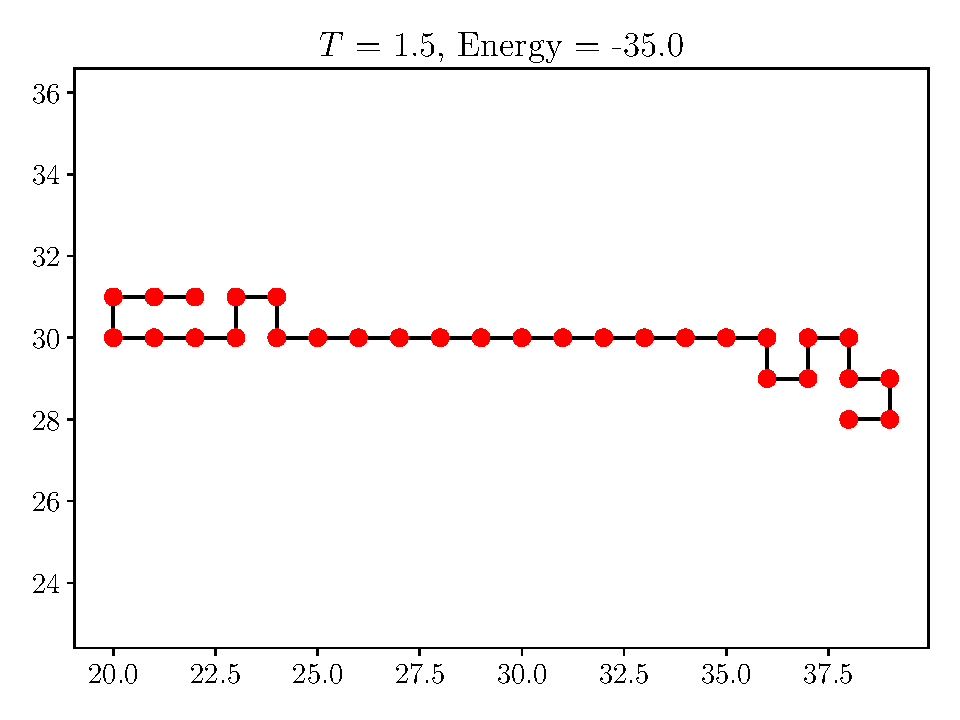
\includegraphics[scale=0.6]{images/Q3a_final_protein_T15_N30_n100000.pdf}}
    \caption{The final protein structure for the initial parameters. }.
    \label{fig:q3a_protein1}
\end{figure}
\begin{figure}[h!]
    \centerline{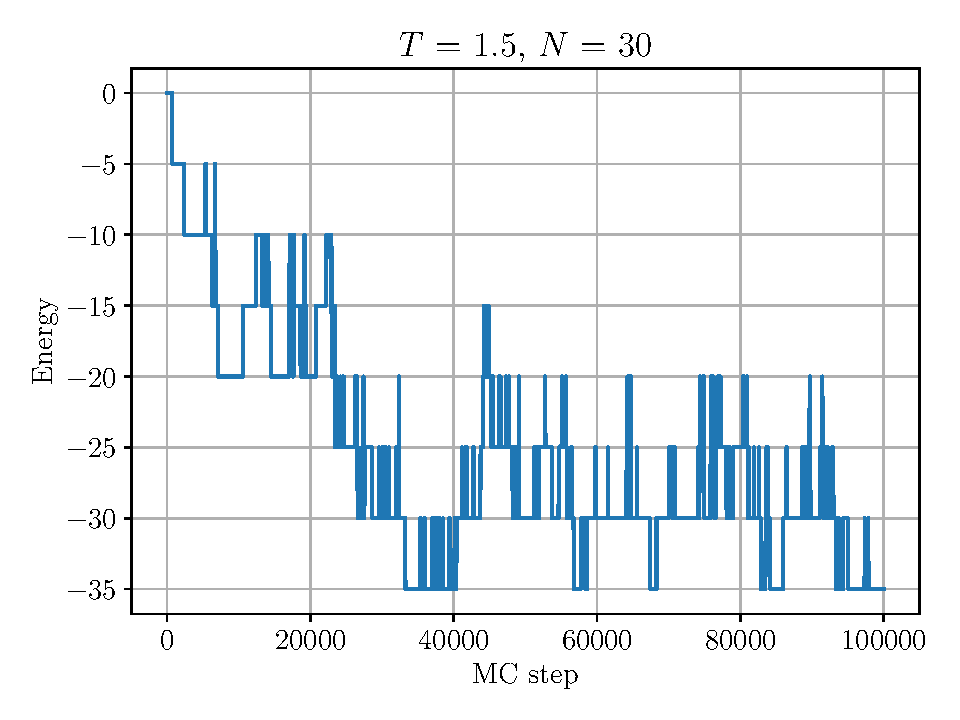
\includegraphics[scale=0.6]{images/Q3a_energy_vs_step_T15_N30_n100000.pdf}}
    \caption{The energy versus montecarlo step for the same run as Fig \ref{fig:q3a_protein}. }.
    \label{fig:q3a_energy1}
\end{figure}

We change the temperature $T =0.5$ and run the script again. We get Fig \ref{fig:q3a_protein0.5} and \ref{fig:q3a_energy0.5} respectively. \\
\begin{figure}[h!]
    \centerline{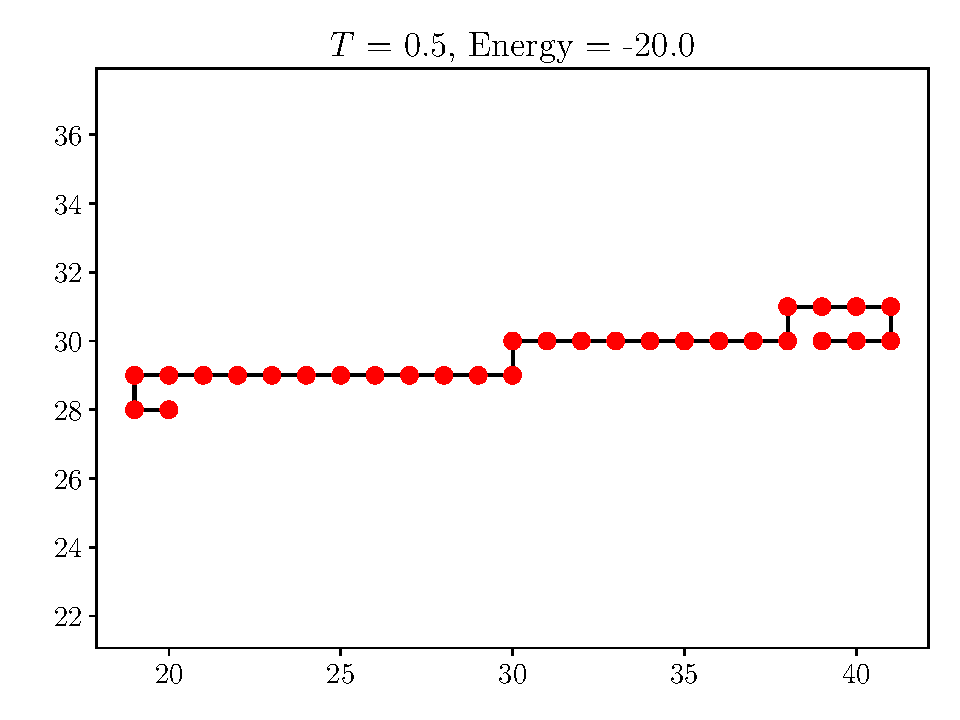
\includegraphics[scale=0.6]{images/Q3a_final_protein_T5_N30_n100000.pdf}}
    \caption{The final protein structure for the initial parameters. }.
    \label{fig:q3a_protein0.5}
\end{figure}
\begin{figure}[h!]
    \centerline{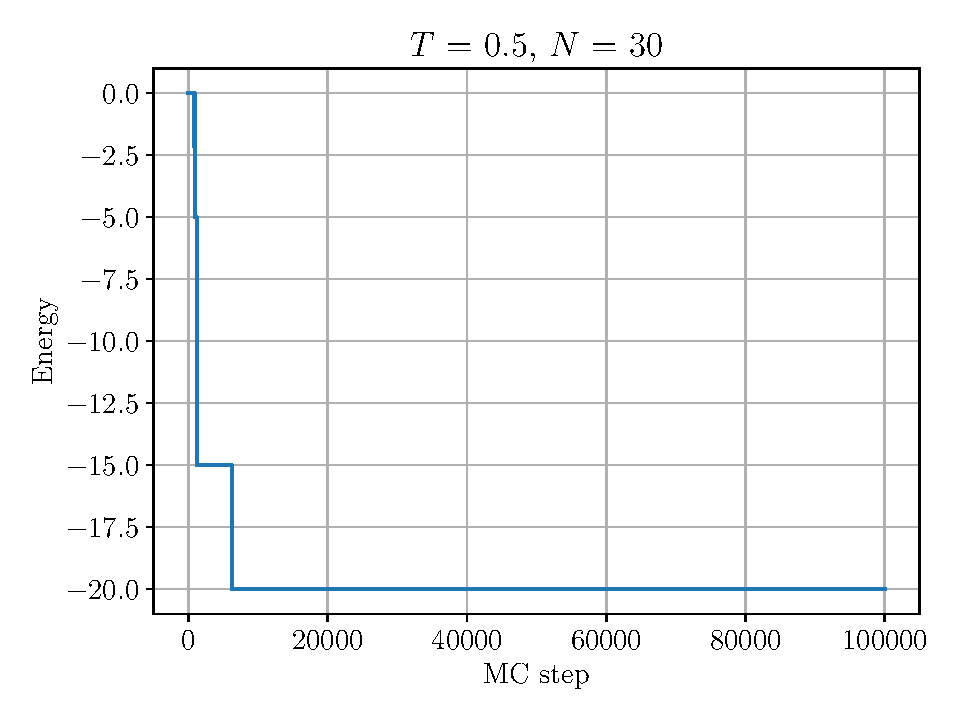
\includegraphics[scale=0.6]{images/Q3a_energy_vs_step_T5_N30_n100000.pdf}}
    \caption{The energy versus montecarlo step for the same run as Fig \ref{fig:q3a_protein0.5}. }.
    \label{fig:q3a_energy0.5}
\end{figure}

We change the temperature $T =5.0$ and run the script again. We get Fig \ref{fig:q3a_protein5} and Fig \ref{fig:q3a_energy5} respectively. 
\begin{figure}[h!]
    \centerline{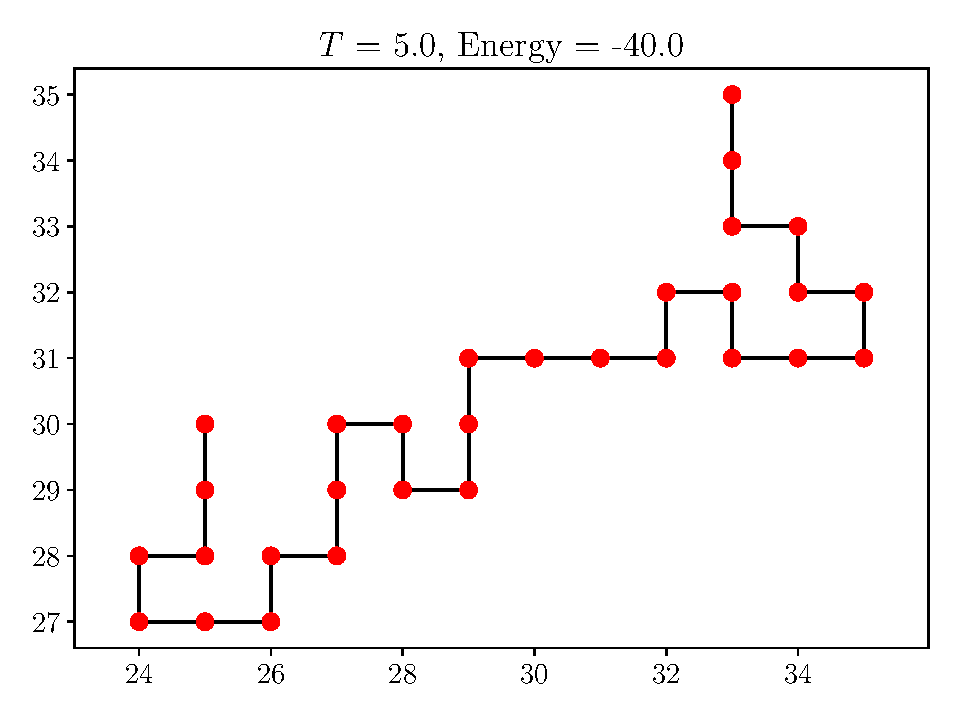
\includegraphics[scale=0.6]{images/Q3a_final_protein_T50_N30_n100000.pdf}}
    \caption{The final protein structure for the initial parameters. }.
    \label{fig:q3a_protein5}
\end{figure}
\begin{figure}[h!]
    \centerline{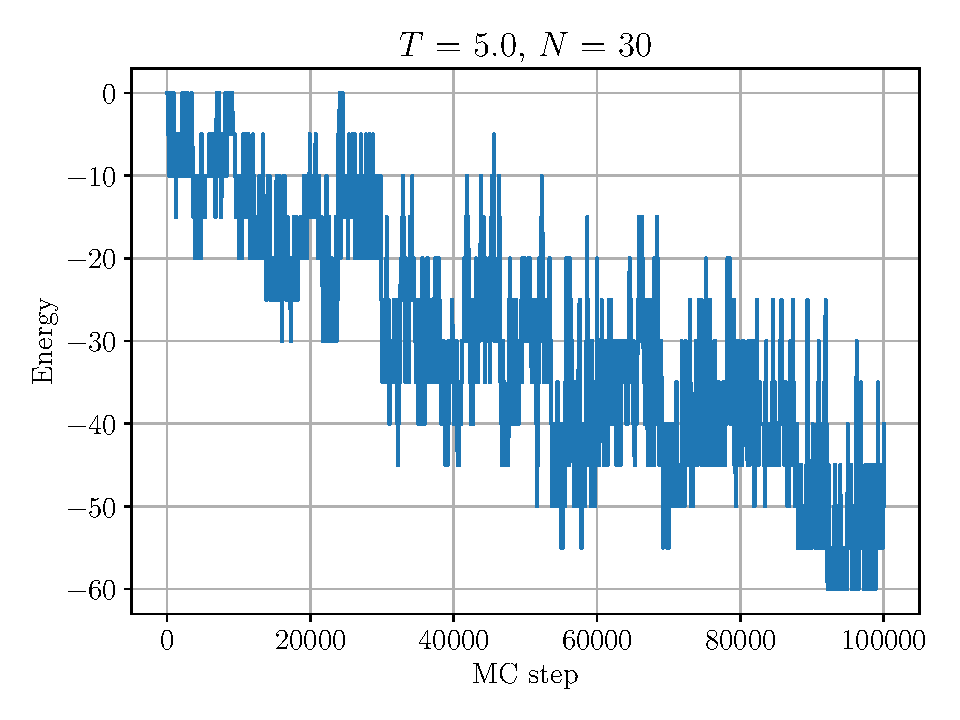
\includegraphics[scale=0.6]{images/Q3a_energy_vs_step_T50_N30_n100000.pdf}}
    \caption{The energy versus montecarlo step for the same run as Fig \ref{fig:q3a_protein5}. }.
    \label{fig:q3a_energy5}
\end{figure}



We see that the proteins have the tendency to spread out as $T$ increases; we can see that the protein obtained for $T = 5$ in Fig \ref{fig:q3a_energy5} is significantly more folded and spread out than that of in Figs \ref{fig:q3a_protein1} and \ref{fig:q3a_protein0.5}, where they appear more folded 'into themselves'. The energy fluctuates more as $T$ increases: we have a relatively stable energy states for long periods of steps for T = 0.5, a descent with fluctuations when T = 1.5 and extreme fluctuations with a decreasing pattern when T =5.0. We note that the energy minimas appear lower for the higher values of T from our three graphs. 


\subsection*{b)}
We are instructed to consider $n = 1000,000$ steps this time and consider $T = 1.5$ and $T =0.5$. To do this, we simply modify the $n$ parameter in the code. 

We consider $T=1.5$ first. In this case, the average energy over the second half is -55.77 (obtained from the printed output). The plots for the final protein structure and the energy can be seen in Fig \ref{fig:q3b_protein15} and \ref{fig:q3b_energy15}. We then consider $T = 0.5$. In this case the average energy over the second half is -15.00, while the protein structure can be seen in Fig \ref{fig:q3b_protein5} and its energy in Fig \ref{fig:q3b_energy5}. 

We can see for lower temperature $T = 0.5$ the average energy for the second half of the simulation is significantly lower. This is also evident in the final states of the proteins: the final state for $T = 0.5$ in Fig \ref{fig:q3b_protein5} adopts a less energetic folded in position compared to that of $T = 1.0$, which as a more spread out position \ref{fig:q3b_protein5}. 

We expect this. When $T$ becomes smaller, the Boltzman factor $\exp{- \Delta E/ \Delta T}$ becomes larger. Thus, should the proposed state be a more energetic position, the move is more likely to be larger than our randomly generated number between 0 and 1; its more likely to be accepted. Thus, it is far more likely to see the protein in a higher environment enter more energetic states as we have seen from lower energy states.  


\section*{c)}
We are asked to decrease the temperature over the course of our simulation. We use the hint provided in the question and modify the constants used in the code as follows:
\begin{verbatim}
    eps = -5.0  # interaction energy
    N = 30  # length of protein
    T_f = 0.5  # temperature for Monte Carlo
    n = int(2e6)  # number of Monte Carlo steps
    T_steps = 4
    T_i = T_f + T_steps - 1
    T_array = np.zeros(n)
    for step in range(T_steps):
        T_array[step*n//T_steps:(step+1)*n//T_steps] = \
            (T_i-T_f)*(1-step/(T_steps-1)) + T_f

energy_array = np.zeros(n)  # initialize array to hold energy

\end{verbatim}
We also modify line 135 to \texttt{if random() < np.exp(-(new_energy-energy)/T_array[j]):}/
We also slightly modify the code at the end of the script to average the energy over the last quarter of the simulation when T = 0.5 as requested. We find that the energy averaged over last quarter of simulations is: -70.00. This is significantly lower than the final energy found in part b. We can justify this because the simulated annealing provided a much slower decrease in temperature which allowed the algorithm to find the global minimum as opposed the local minimum 


\section*{d)}
We are asked to further explore the temperature and energy dependence. We modify the script by running 500000 steps of the simulation at each temperature from 10 to 0.5, decreasing the temperature by 0.5. 
In figure \ref{fig:3d} we look for evidence for a phase transition. We notice that that between temperature 8.8 and 6 we have a steady decreasing slope, between temperature 6 and 4.5 we have a slope close to 0, and again a sharp slope between 4.5 and 3.5. Looking at this graph I would predict that a phase transition occurs between T=4.5 and T=3.5 since we see that energy being almost constant before that (we need a significant energy decrease before we can switch phases).

\begin{figure}[H]
    \centerline{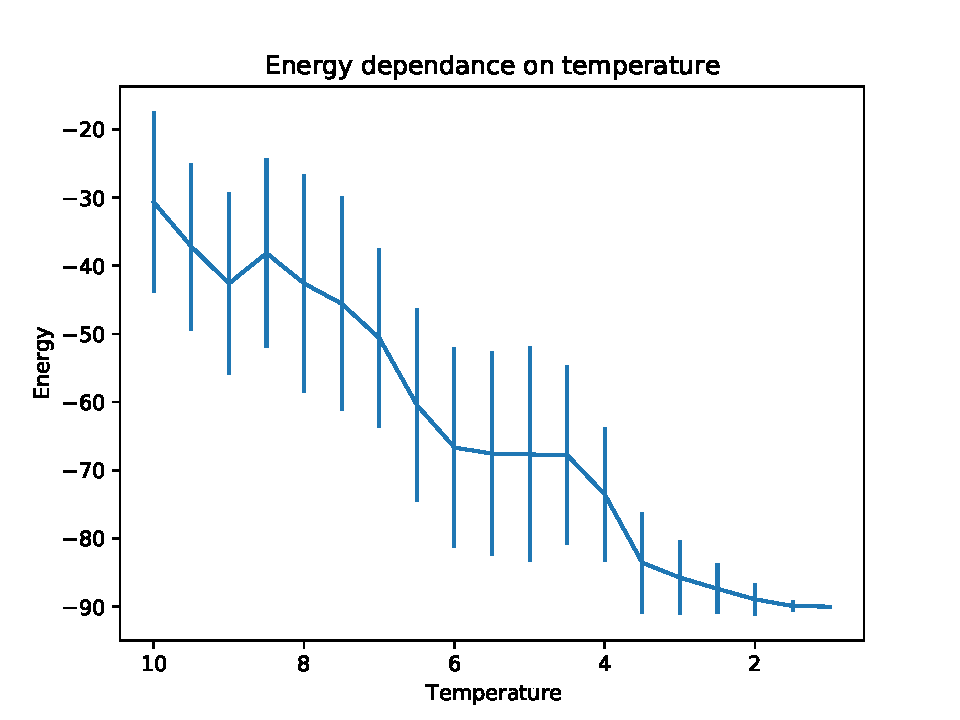
\includegraphics[scale=0.6]{images/Q3d_iii.pdf}}
    \caption{Energy vs temperature, where the energy is the average energy for the that temperature during 500000 simulation steps, error bars represent the standard deviation for each mean.}
    \label{fig:3d}
\end{figure}

\begin{figure}[h!]
    \centerline{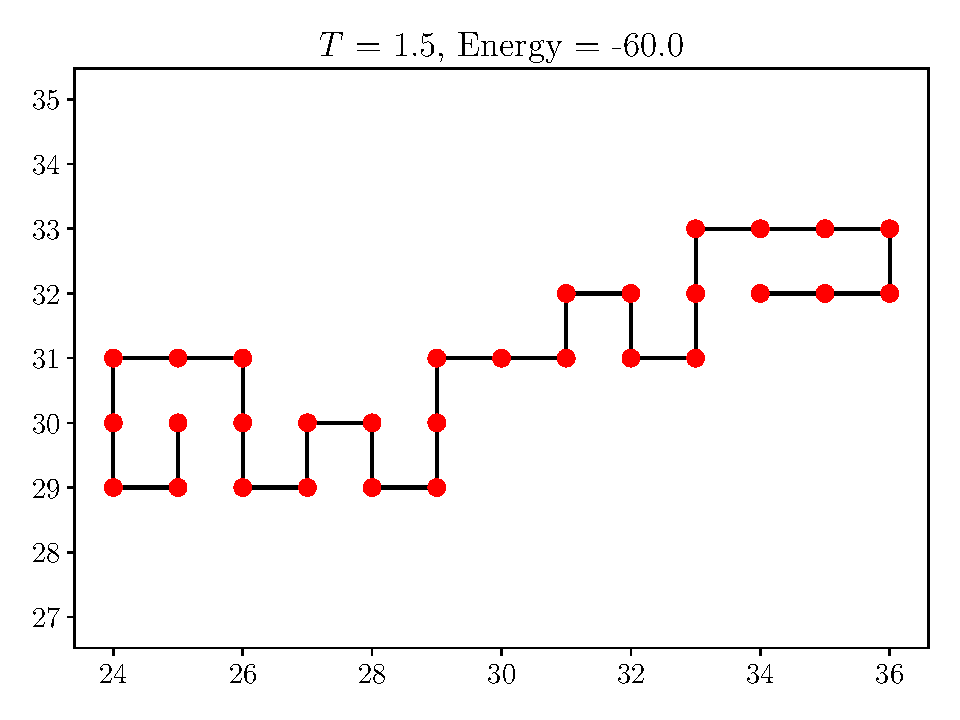
\includegraphics[scale=0.6]{images/Q3b_final_protein_T15_N30_n1000000.pdf}}
    \caption{The final protein structure for the initial parameters. }.
    \label{fig:q3b_protein15}
\end{figure}
\begin{figure}[h!]
    \centerline{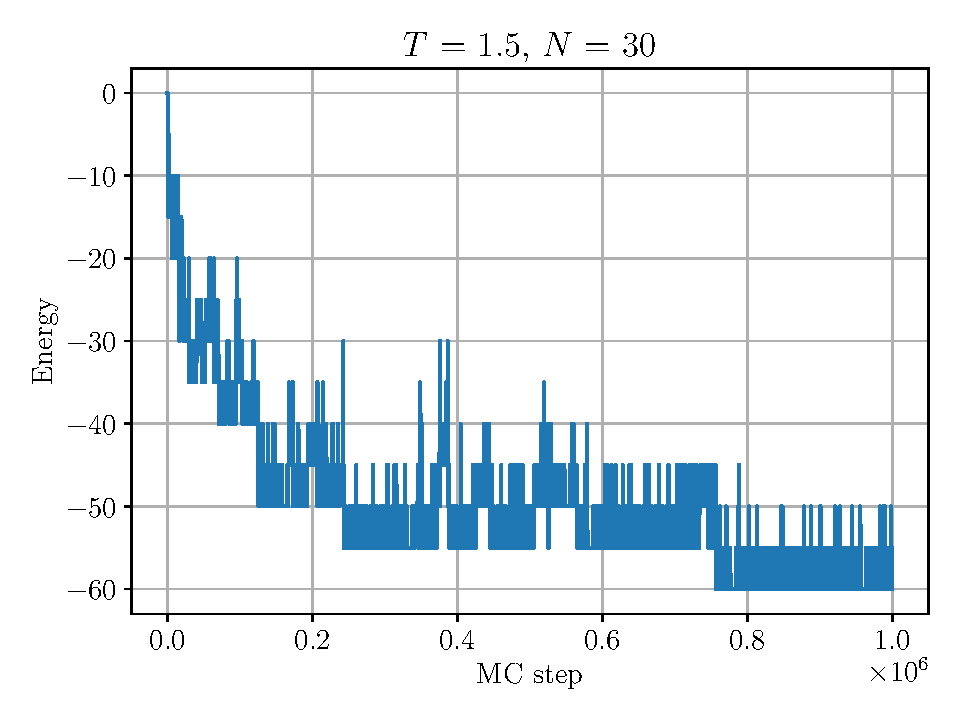
\includegraphics[scale=0.6]{images/Q3b_energy_vs_step_T15_N30_n1000000.pdf}}
    \caption{The energy versus montecarlo step for the same run as Fig \ref{fig:q3b_protein15}. }.
    \label{fig:q3b_energy15}
\end{figure}

\begin{figure}[h!]
    \centerline{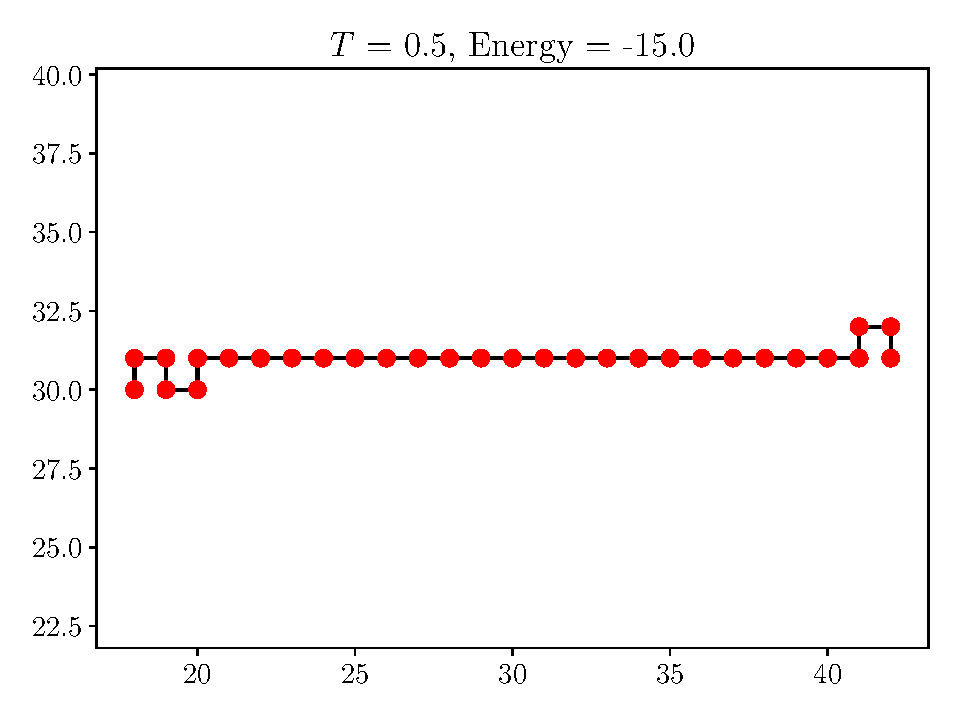
\includegraphics[scale=0.6]{images/Q3b_final_protein_T5_N30_n1000000.pdf}}
    \caption{The final protein structure for the initial parameters. }.
    \label{fig:q3b_protein5}
\end{figure}
\begin{figure}[h!]
    \centerline{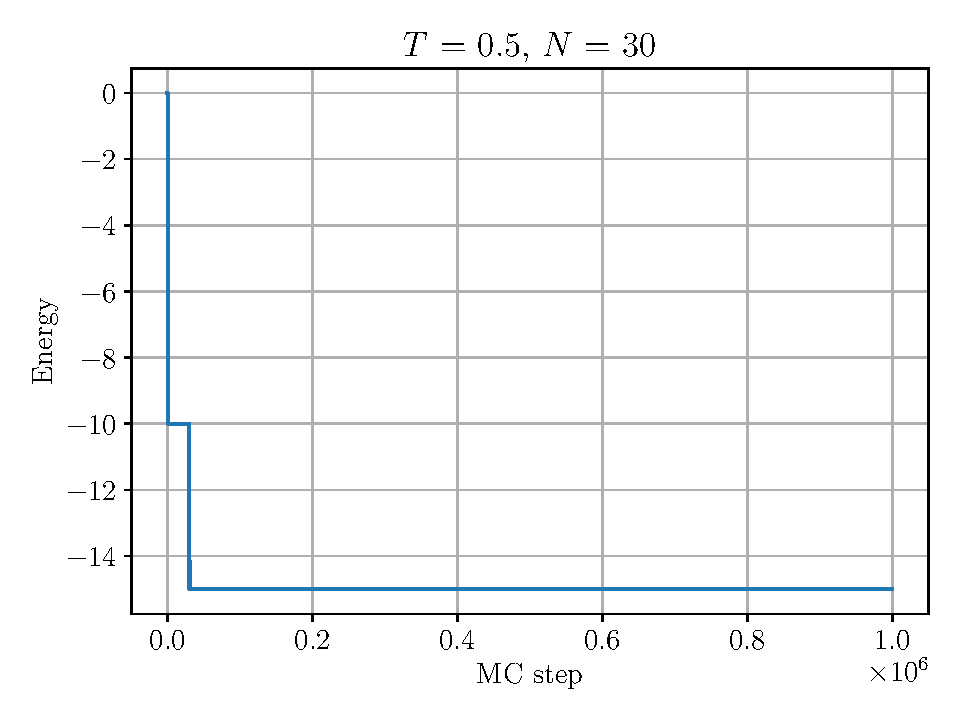
\includegraphics[scale=0.6]{images/Q3b_energy_vs_step_T5_N30_n1000000.pdf}}
    \caption{The energy versus montecarlo step for the same run as Fig \ref{fig:q3b_protein5}. }.
    \label{fig:q3b_energy5}
\end{figure}


% just to set the appendix real Far back
\newpage
\hfill
\newpage
\hfill
\newpage
\section*{Appendix}
\subsection*{Q2c) Figures}
Fig \ref{fig:q2d_magnet_1} to Fig \ref{fig:q2d_magnet_3} the resultant magnetization plots described in question 2 over multiple runs. 
\begin{figure}[H]
    \centerline{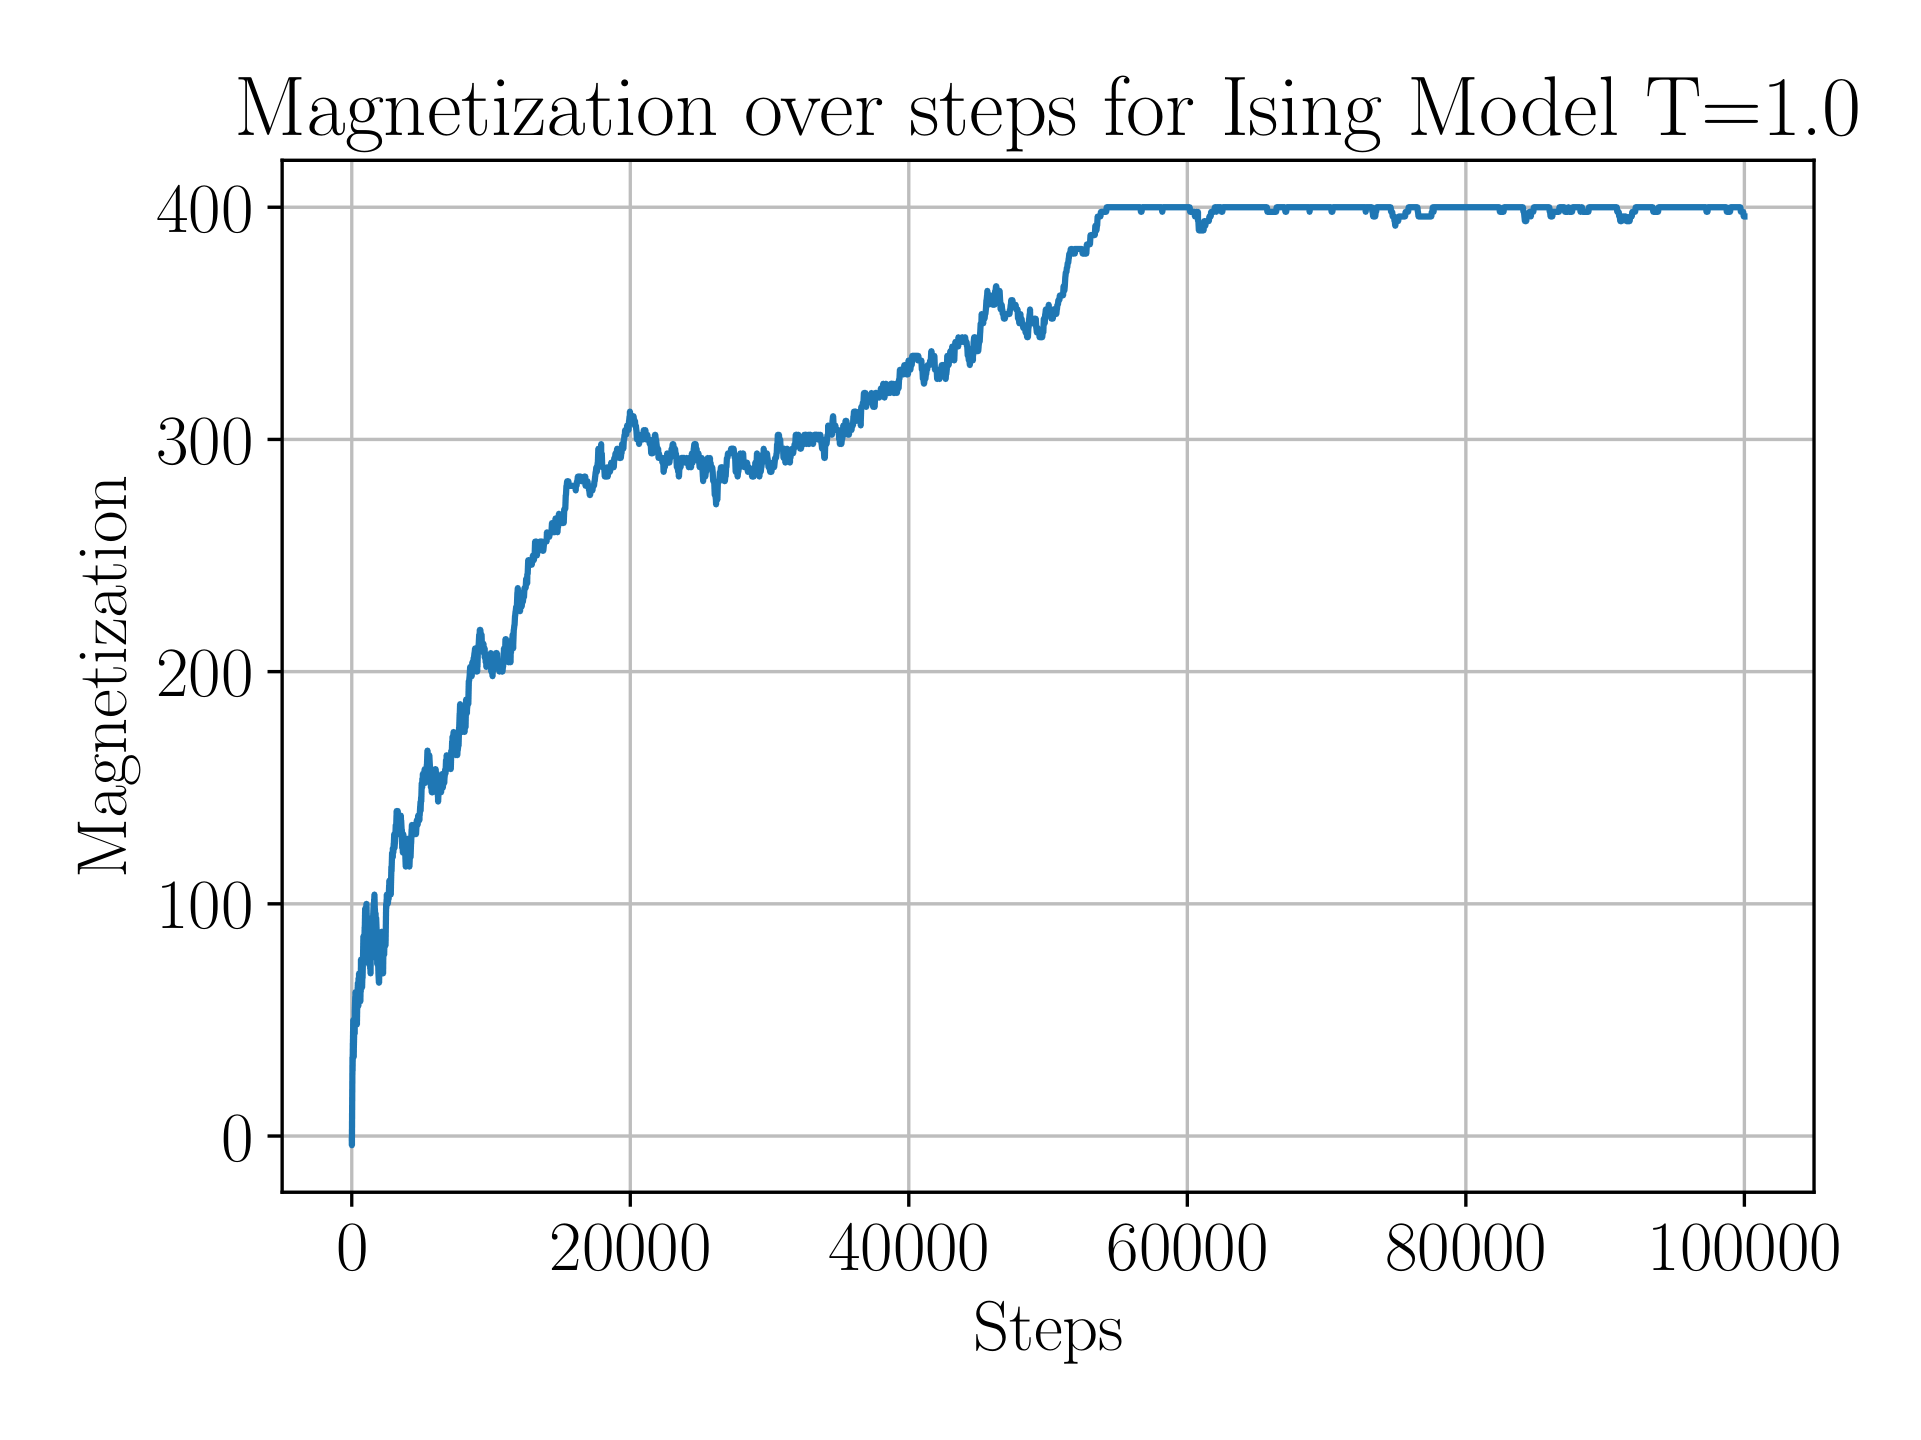
\includegraphics[scale=0.6]{images/Q2_magnetizationT_1.0_3.png}}
    \caption{The Magnetization over the number of steps for our first run of the script. We note this converges to 400.}.
    \label{fig:q2d_magnet_1}
\end{figure}
\begin{figure}[h!]
    \centerline{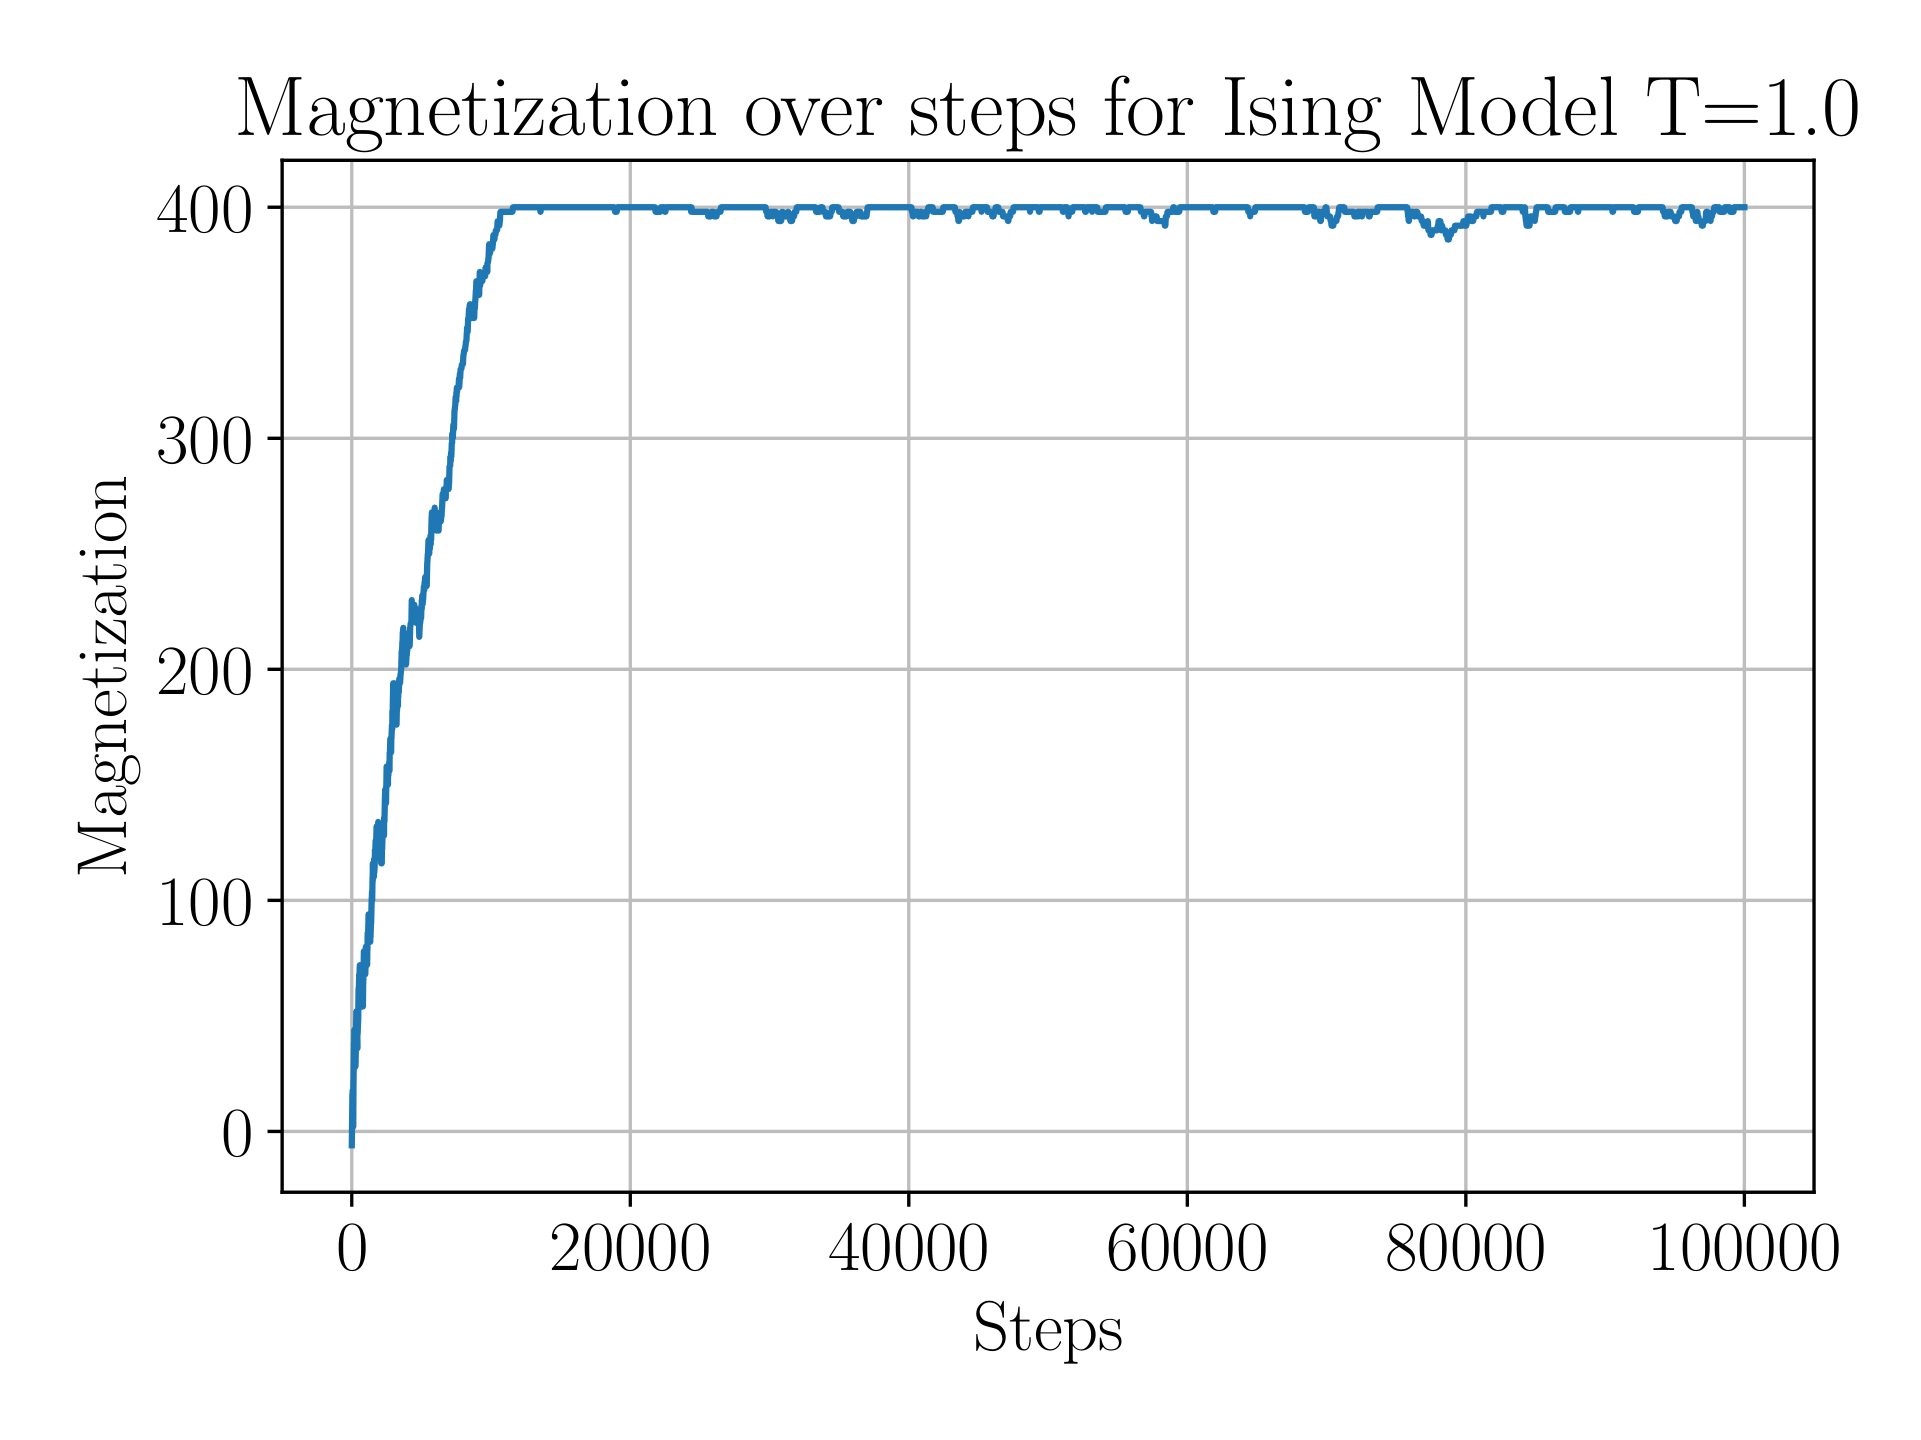
\includegraphics[scale=0.6]{images/Q2_magnetizationT_1.0_4.png}}
    \caption{The Magnetization over the number of steps for our second run of the script. We note this converges to 400.}.
    \label{fig:q2d_magnet_2}
\end{figure}
\begin{figure}[h!]
    \centerline{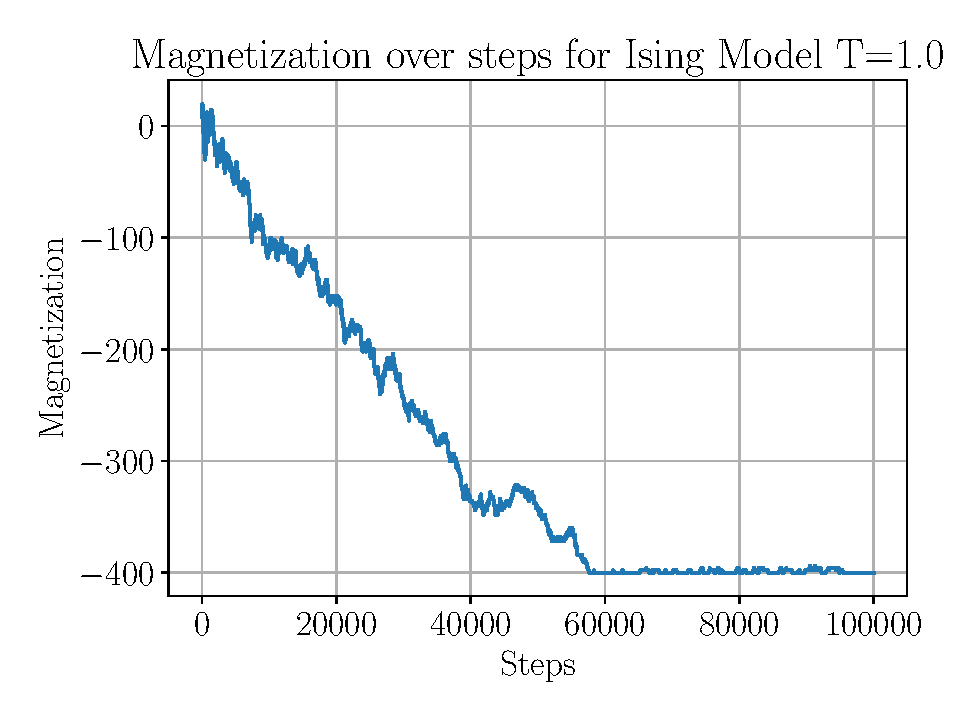
\includegraphics[scale=0.6]{images/Q2_magnetizationT_1.0_5.p}}
    \caption{The Magnetization over the number of steps for our third run of the script. We note this converges to -400.}.
    \label{fig:q2d_magnet_3}
\end{figure}




\end{document}
